%%This is a very basic article template.
%%There is just one section and two subsections.
\documentclass{article}

\usepackage{mathtools}
\usepackage{graphicx}

\title{Homework 3}
\author{Steve Hill}



\begin{document}
\vspace*{-1in}
\huge
\begin{center}
Homework 3

Steve Hill
\end{center}
\normalsize

\section{Problem 1}
Define functional margin and geometric margin. Explain why functional margin is not a 
good objective to optimize in order to learn a maximum margin classifier:


Functional Margin - Functional margin is the margin defined by wx + b = 0.
So if you multiply some point yi by the functional margin, you should get a
classifier such that if classifier > 0 then it is positive.


The problem comes if the bound is too tightly fit, we want things to fit better,
so we should look to expand the margin.


Geometric Margin - The geometric margin is a wider margin respresented by the
first useful example points in each class. By fitting two margins, wx + b = 1
and wx + b = -1, we can create a wider margin that is as large as possible.
This is what we want.

\section{Problem 2}
For the soft-margin SVM, parameter c controls the trade-off between maximizing the 
margin and minimizing the slack variables (aka the ‘error’ of the fat decision boundary). 
Consider the following data set, what linear decision boundary will soft-margin SVM 
learn when:\newline

\noindent
Note that the outmost boundries are the fat boundry for each c value.
\begin{center}
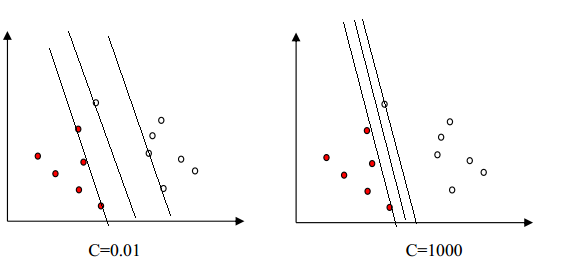
\includegraphics[scale = .6]{SVMex.png}
\end{center}
\section{Problem 3}

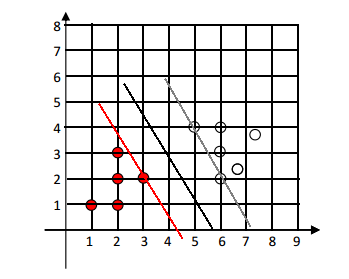
\includegraphics[scale = .6]{Kmeans1.png}

\[Gray = wx + b = 1\] 
\[Red = wx + b = -1\] 
\[Black = wx + b\ = 0\]

\noindent Part b) The Gray and Red lines represent two support vectors 
\newline\newline
Part c) The w value is (1, 2) and the b value is 10.
\newpage
\section{Problem 4}
Data set: (-1.8, -1.7, -0.3, -.1, 0.2, 0.4, 1.6, 1.7, 1.9, 2.0)
\newline\noindent Dendograms:
\begin{center}
Single Link Clusters
\end{center}
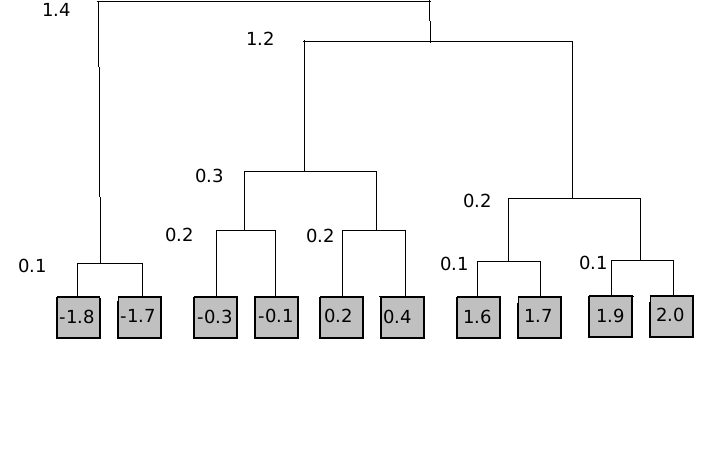
\includegraphics[scale = .5]{SingleLinkBox.png}
\begin{center}
Complete Link Clusters
\end{center}
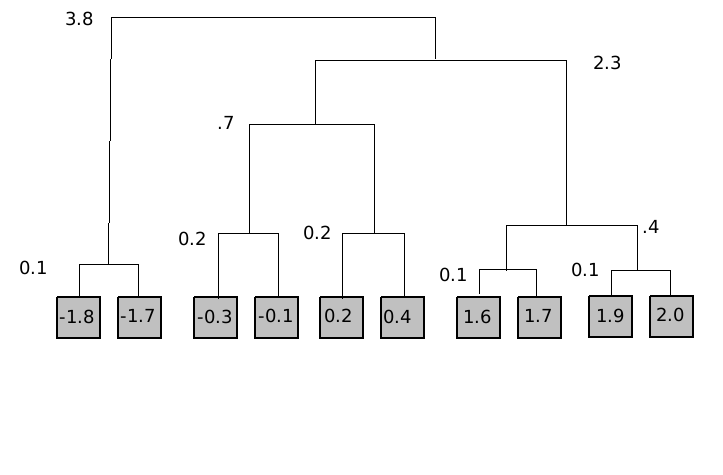
\includegraphics[scale = .5]{CompleteLinkBox.png}






\end{document}
